% \PassOptionsToPackage{table}{xcolor}
\documentclass[11pt]{beamer}
\usepackage[utf8]{inputenc}
\usepackage[english]{babel}
\usepackage{amsmath}
\usepackage{amsfonts}
\usepackage{amssymb}
\usepackage{graphicx}
\usepackage{tikz}
\usepackage{algorithm}
\usepackage{algorithmic}
\usepackage{silence,lmodern}
\usepackage{csquotes}
\usepackage[backend=bibtex, bibencoding=ascii, style=authoryear, doi=false, isbn=false,url=false, uniquename=init, giveninits=true]{biblatex}
\usepackage{multimedia}
\usepackage{dirtytalk}
\usepackage{pgfplotstable,booktabs}
\usepackage{grffile}
\usepackage{marvosym} % color image
\WarningFilter{biblatex}{Patching footnotes failed}
\pgfplotsset{compat=newest}


% \mode<presentation>
% {
    \usetheme[hideothersubsections]{PaloAlto}
    % \usecolortheme{beaver}
% }
\usetikzlibrary{calc,trees,positioning,arrows,chains,shapes.geometric,
decorations.pathreplacing,decorations.pathmorphing,
shapes,matrix,shapes.symbols,plotmarks,decorations.markings,
shadows,shapes.geometric,arrows}

\setbeamercolor{logo}{bg=white}  %controls the color of the logo area
\setbeamerfont{footnote}{size=\tiny}

% \addbibresource{library.bib}

\makeatletter
\setlength{\beamer@headheight}{.9cm}
\makeatother

\author{S M Al Mahi}
\title[ECEN-5283 Computer Vision]{Project 6: \\Face Recognition Using\\Principal Component Analysis (\textbf{PCA})}
\setbeamercovered{transparent} 
\setbeamertemplate{navigation symbols}{}


\logo{
\includegraphics[width=1cm]{Oklahoma_State_University_logo.png}}
\institute{Oklahoma State University} 
\date{\today} 
\subject{}
\begin{document}

\setbeamertemplate{sidebar left}{}
\begin{frame}
\titlepage
\end{frame}

\newpage
\setbeamertemplate{sidebar left}[sidebar theme]
\section{Project Objective}
\begin{frame}
\frametitle{Project Objective}
	\begin{block}{Objectives}
	\begin{enumerate}
		\item Implement PCA for face recognition
		\item Reconstructing Images from most important principal components 
		\item Analyze the result with different number of principal components
		\item Apply them to test 120 known and 3 unknown faces and 3 other images
    \item Classification accuracy presented in rank matrix
	\end{enumerate}
	\end{block}
\end{frame}

\section{Technical Background}
\subsection{PCA}
\begin{frame}
\frametitle{PCA}
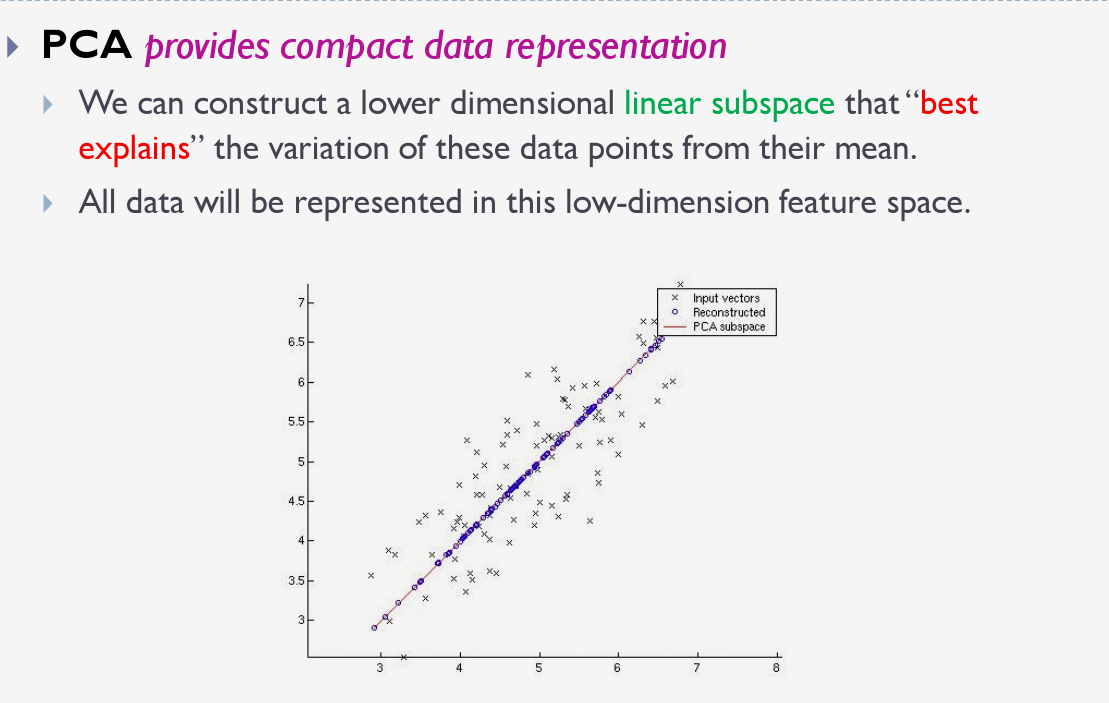
\includegraphics[width=\textwidth]{PCA1.png}
\end{frame}
\begin{frame}
\frametitle{PCA}
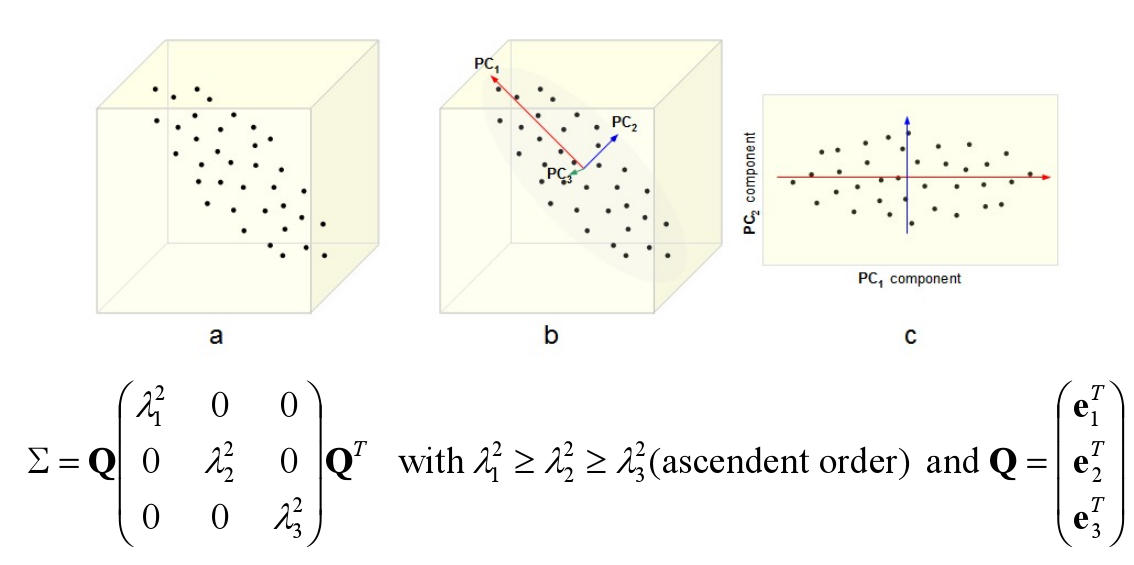
\includegraphics[width=\textwidth]{PCA2.png}
\end{frame}
\subsection{PCA for Face Recognition}
\begin{frame}
\frametitle{PCA}
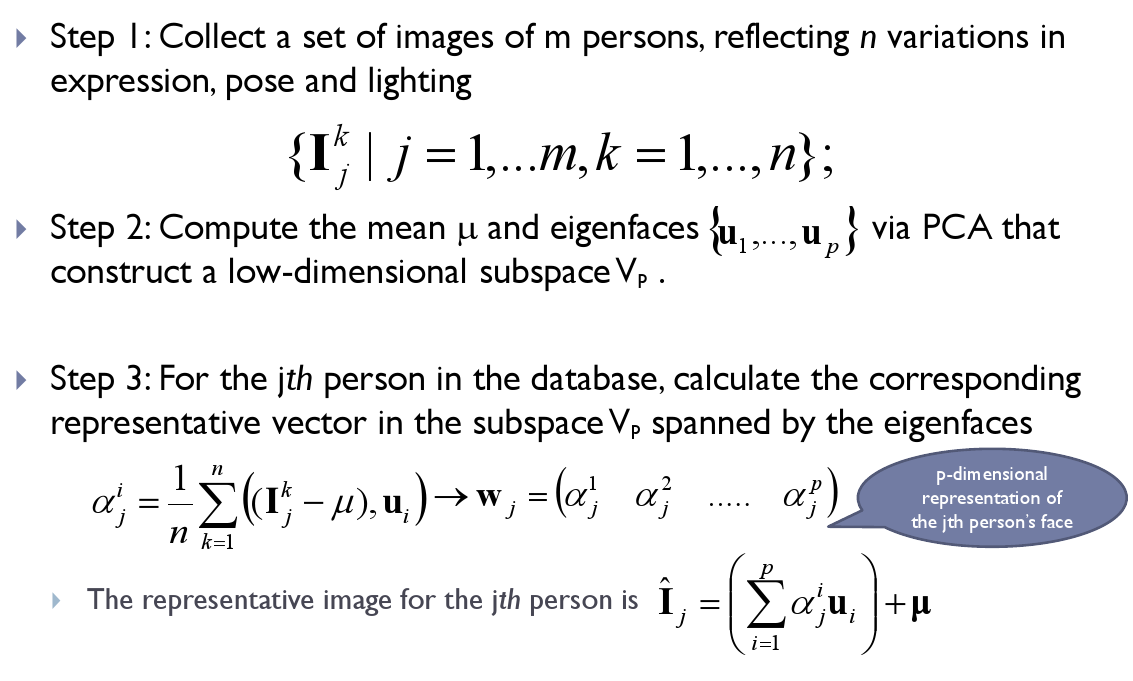
\includegraphics[width=\textwidth]{PCA3.png}
\end{frame}
\begin{frame}
\frametitle{PCA}
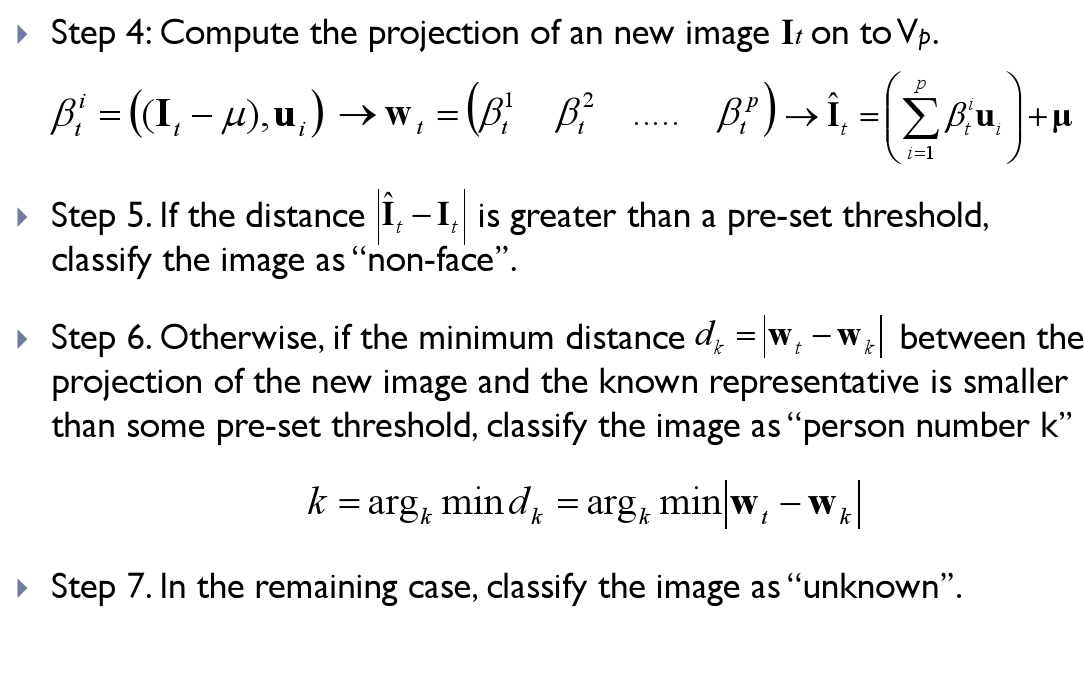
\includegraphics[width=\textwidth]{PCA4.png}
\end{frame}

\section{Analysis of 60 Images in data set}
\subsection{Training}
\begin{frame}
\begin{itemize}
  \item Dataset 60 face images has been divided into two equal training and test sets
  \item Analysis has been performed to training set for Eigen properties and Statistics
  \item Test set is used for classification accuracy and rank matrix
  \item Additional test images were used for non-face and unknown face input.
\end{itemize}
\end{frame}
\begin{frame}
\frametitle{Progressive Increase of Sum of Eigen Values}
\begin{figure}
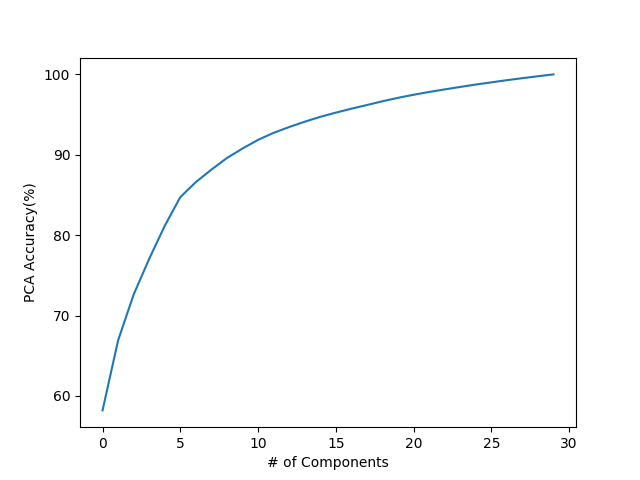
\includegraphics[width=.8\textwidth]{PCA_accuracy.png}
\caption{Progressive Increase in sum of eigne values aka PCA accuracy shows that with only 7 principal 
component it get more than 90\% accuracy. It converges to around 99\% with Principal Component 30.}
\end{figure}
\end{frame}

\begin{frame}
\frametitle{Progressive Decrease in Eigen Values}
\begin{figure}
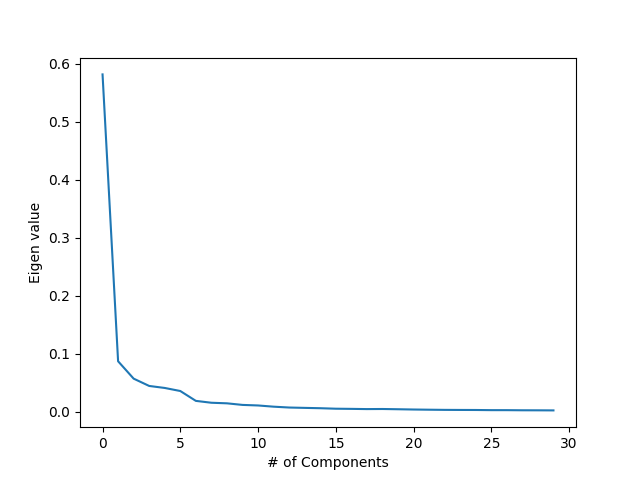
\includegraphics[width=.8\textwidth]{Eigen_values.png}
\caption{Progressive Decrease in Eigen values suggest that around 18 principal component can produce fairly good result.}
\end{figure}
\end{frame}

\begin{frame}
\frametitle{Mean Faces for Test Faces}
\begin{figure}
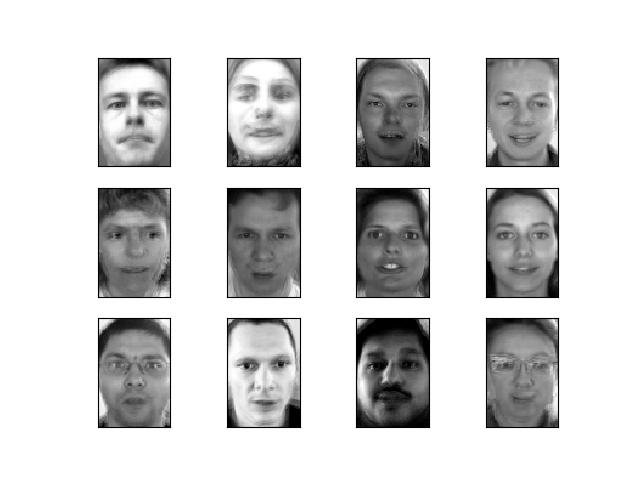
\includegraphics[width=.95\textwidth]{mean_image.png}
\end{figure}
\end{frame}

\begin{frame}
\frametitle{Top Eigen Faces with 3 Principal Component}
\begin{figure}
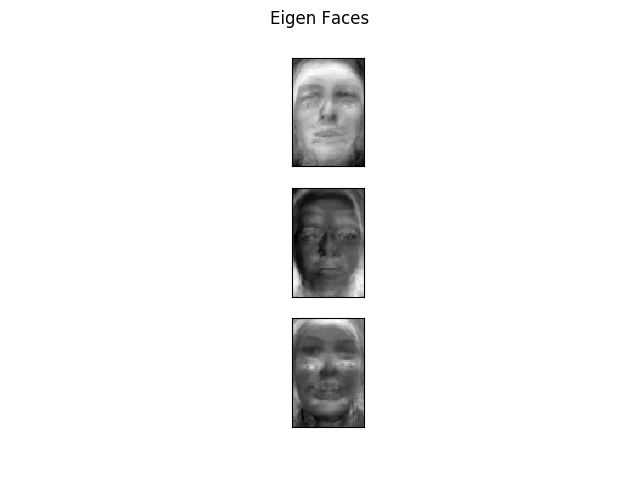
\includegraphics[width=.95\textwidth]{eigen_face_U_3.png}
\end{figure}
\end{frame}

\begin{frame}
\frametitle{Top Eigen Faces with 9 Principal Component}
\begin{figure}
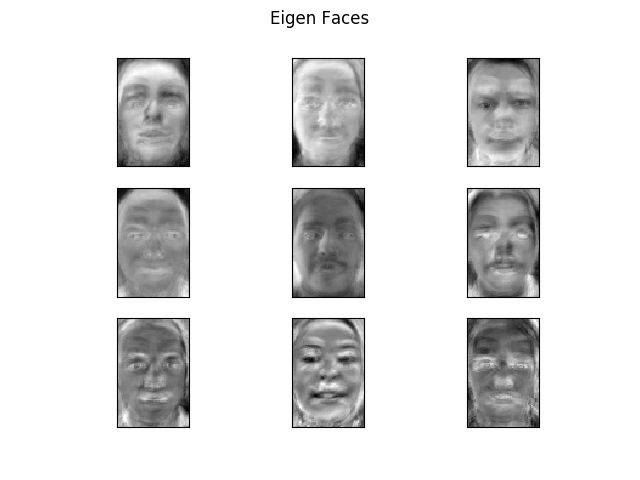
\includegraphics[width=.95\textwidth]{eigen_face_U_9.png}
\end{figure}
\end{frame}

\begin{frame}
\frametitle{Top Eigen Faces with 18 Principal Component}
\begin{figure}
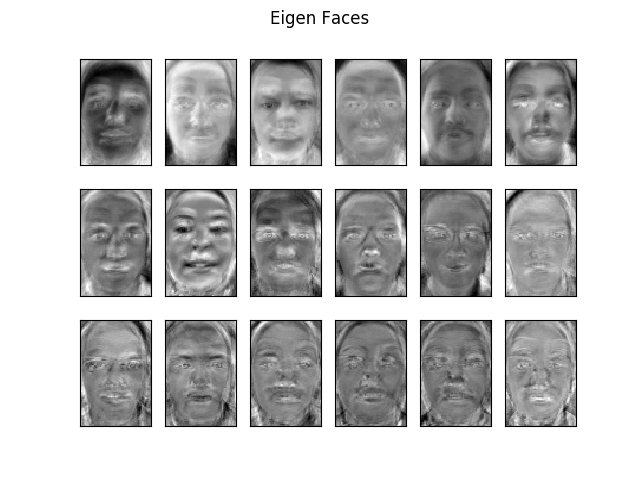
\includegraphics[width=.95\textwidth]{eigen_face_U_18.png}
\end{figure}
\end{frame}

\begin{frame}
\frametitle{Top Eigen Faces with 72 Principal Component}
\begin{figure}
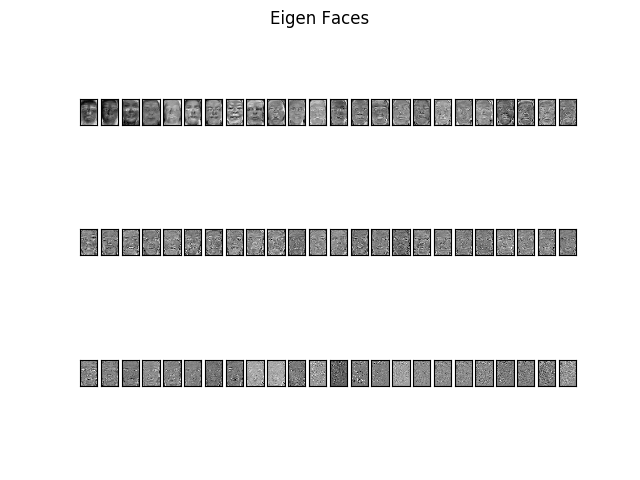
\includegraphics[width=.8\textwidth]{eigen_face_U_72.png}
\caption{Many of the Eigen face mostly looks like noise. Means that they have least significance in classification.}
\end{figure}
\end{frame}

\section{PCA Reconstruction}
\begin{frame}
\frametitle{PCA reconstruction Using 3 Principal Components}
\begin{figure}
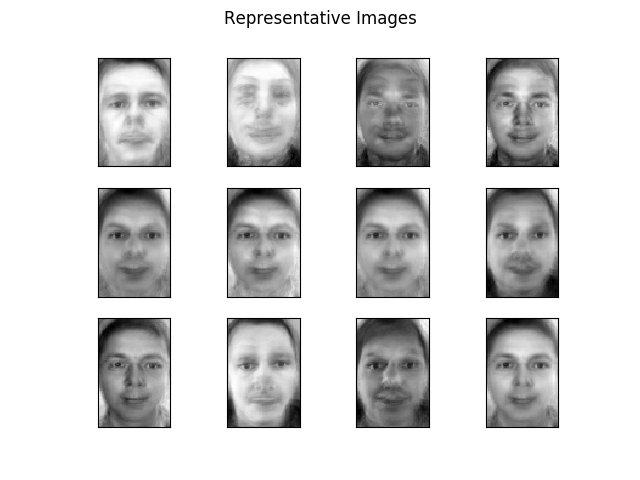
\includegraphics[width=.95\textwidth]{Representative_Images_U_3.png}
\end{figure}
\end{frame}

\begin{frame}
\frametitle{PCA reconstruction Using 9 Principal Components}
\begin{figure}
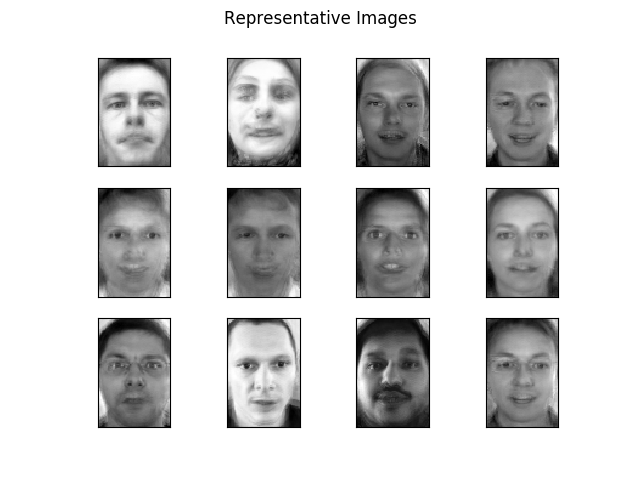
\includegraphics[width=.95\textwidth]{Representative_Images_U_9.png}
\end{figure}
\end{frame}

\begin{frame}
\frametitle{Reconstruction Using 18 Principal Components}
\begin{figure}
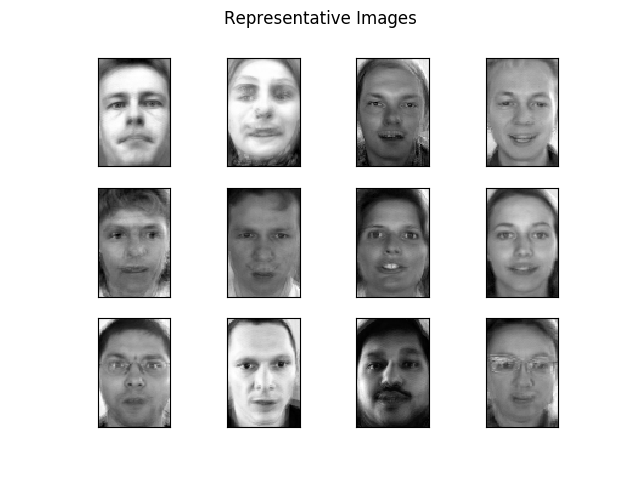
\includegraphics[width=.95\textwidth]{Representative_Images_U_18.png}
\end{figure}
\end{frame}

\begin{frame}
\frametitle{Reconstruction Using 72 Principal Components}
\begin{figure}
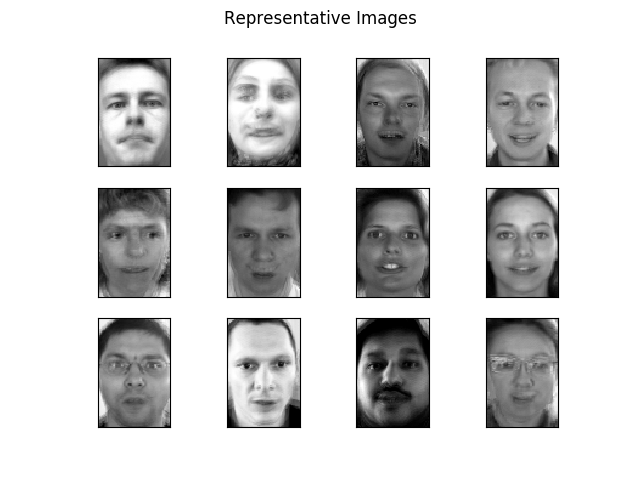
\includegraphics[width=.95\textwidth]{Representative_Images_U_72.png}
\end{figure}
\end{frame}

\begin{frame}
\frametitle{Reconstruction Cost Known Face P=3}
\begin{figure}
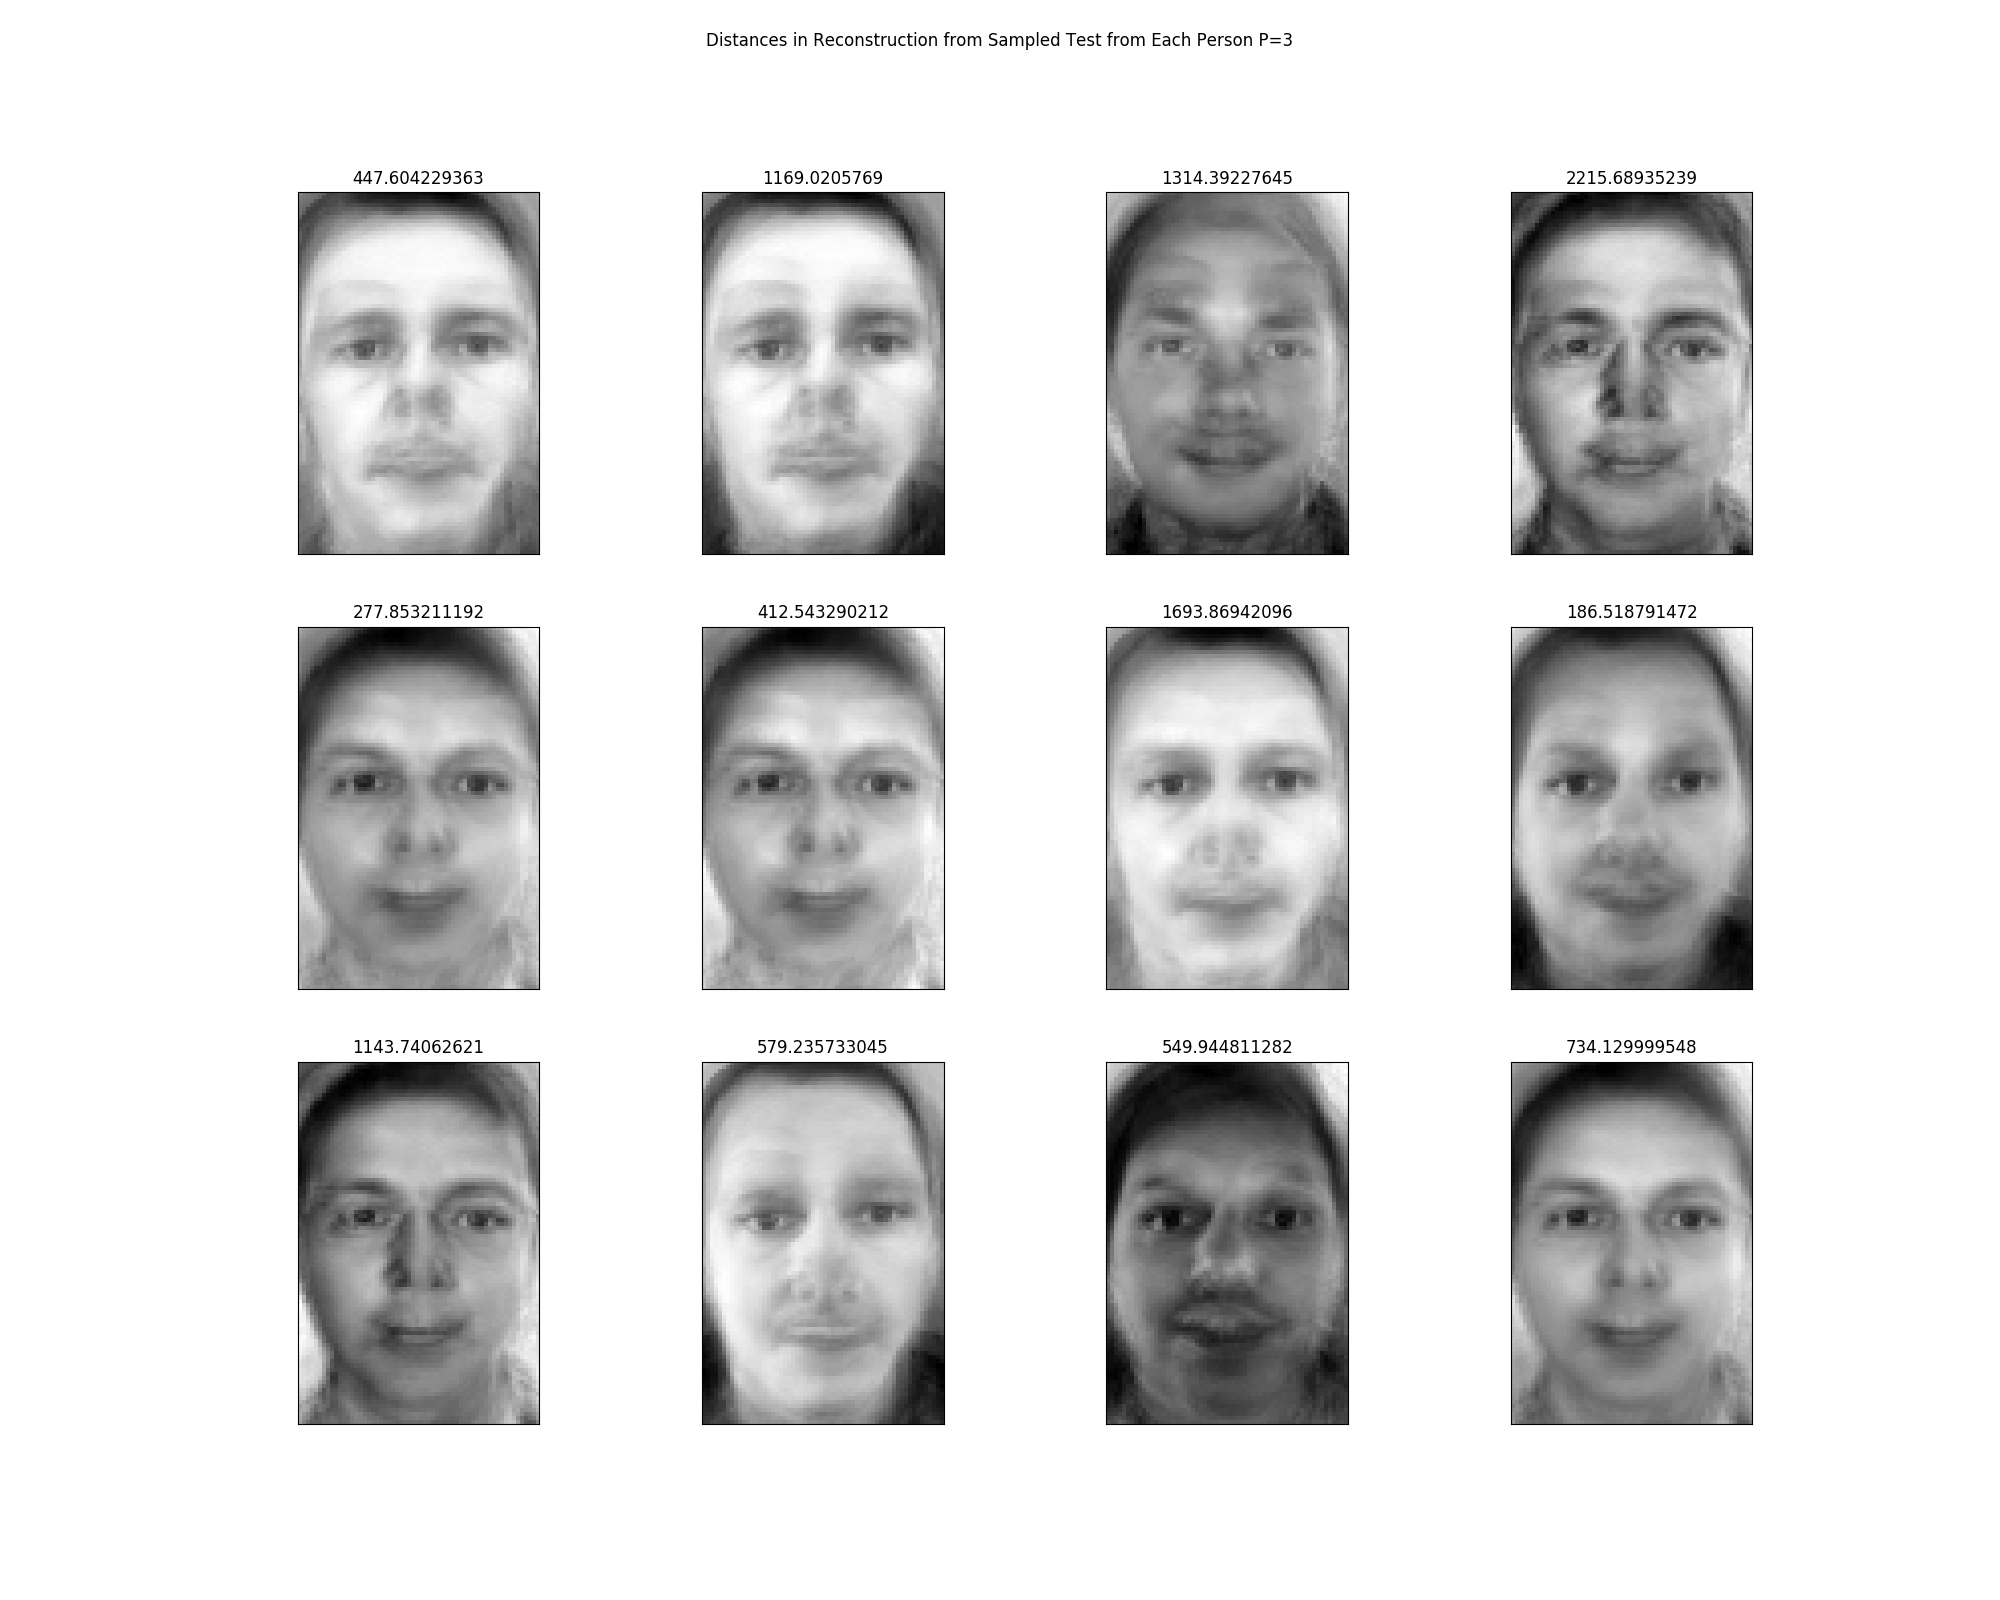
\includegraphics[width=.95\textwidth]{reconstruction_cost_3.png}
\end{figure}
\end{frame}

\begin{frame}
\frametitle{Reconstruction Cost Known Face P=9}
\begin{figure}
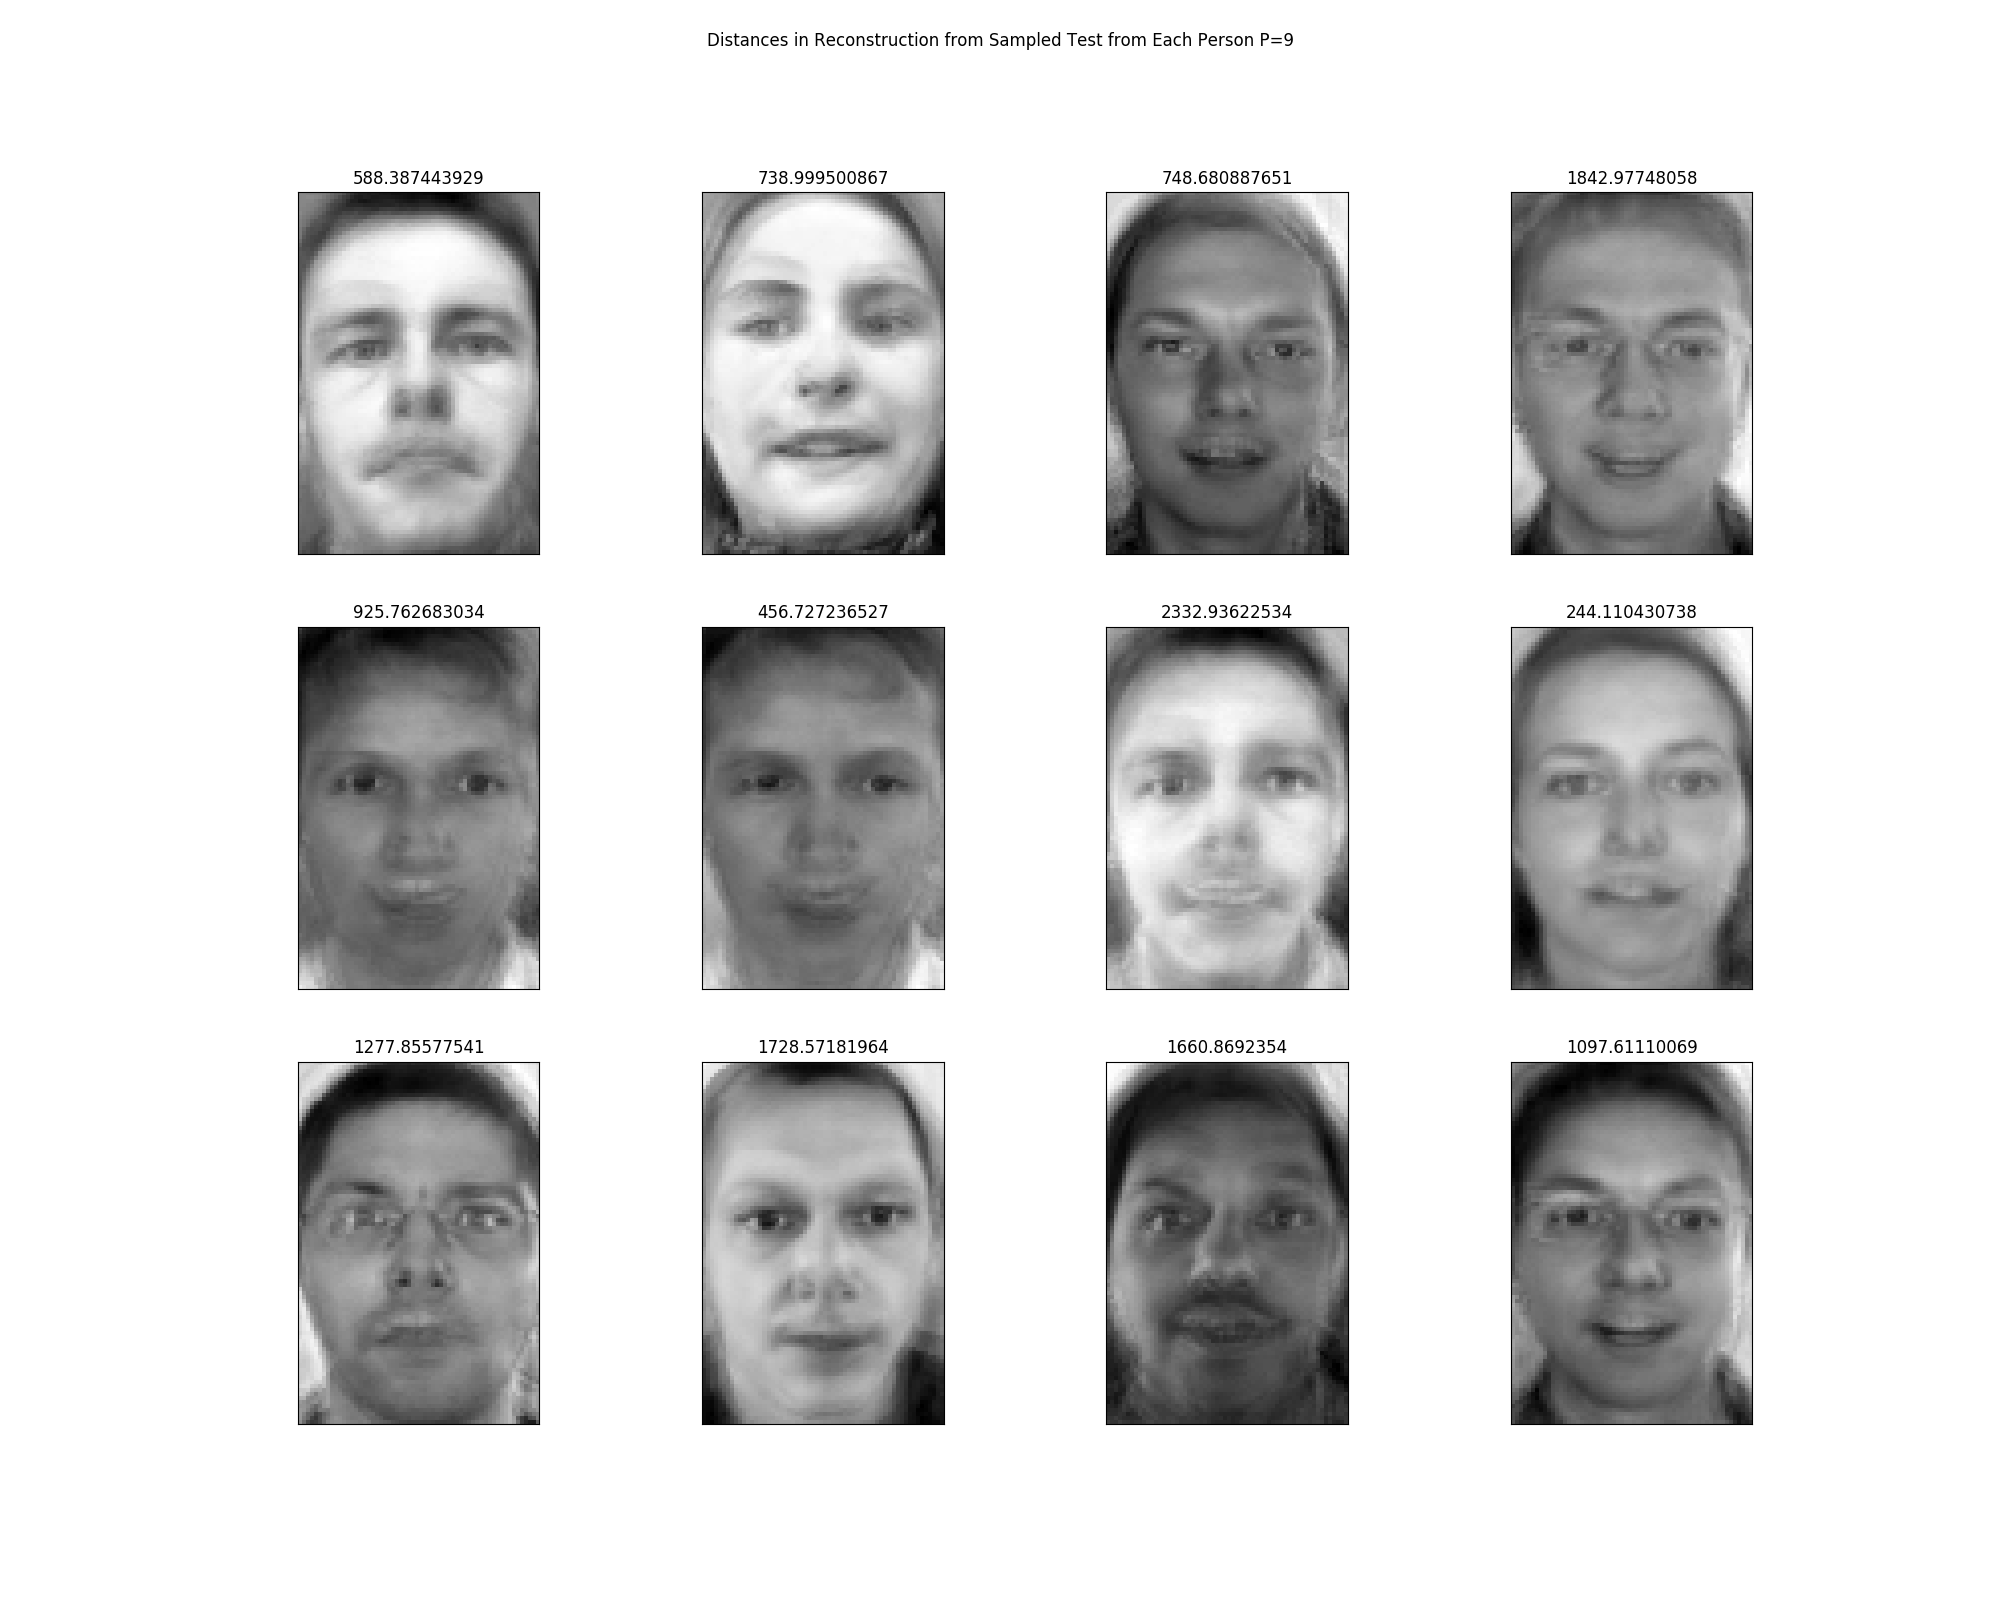
\includegraphics[width=.95\textwidth]{reconstruction_cost_9.png}
\end{figure}
\end{frame}

\begin{frame}
\frametitle{Reconstruction Cost Known Face P=18}
\begin{figure}
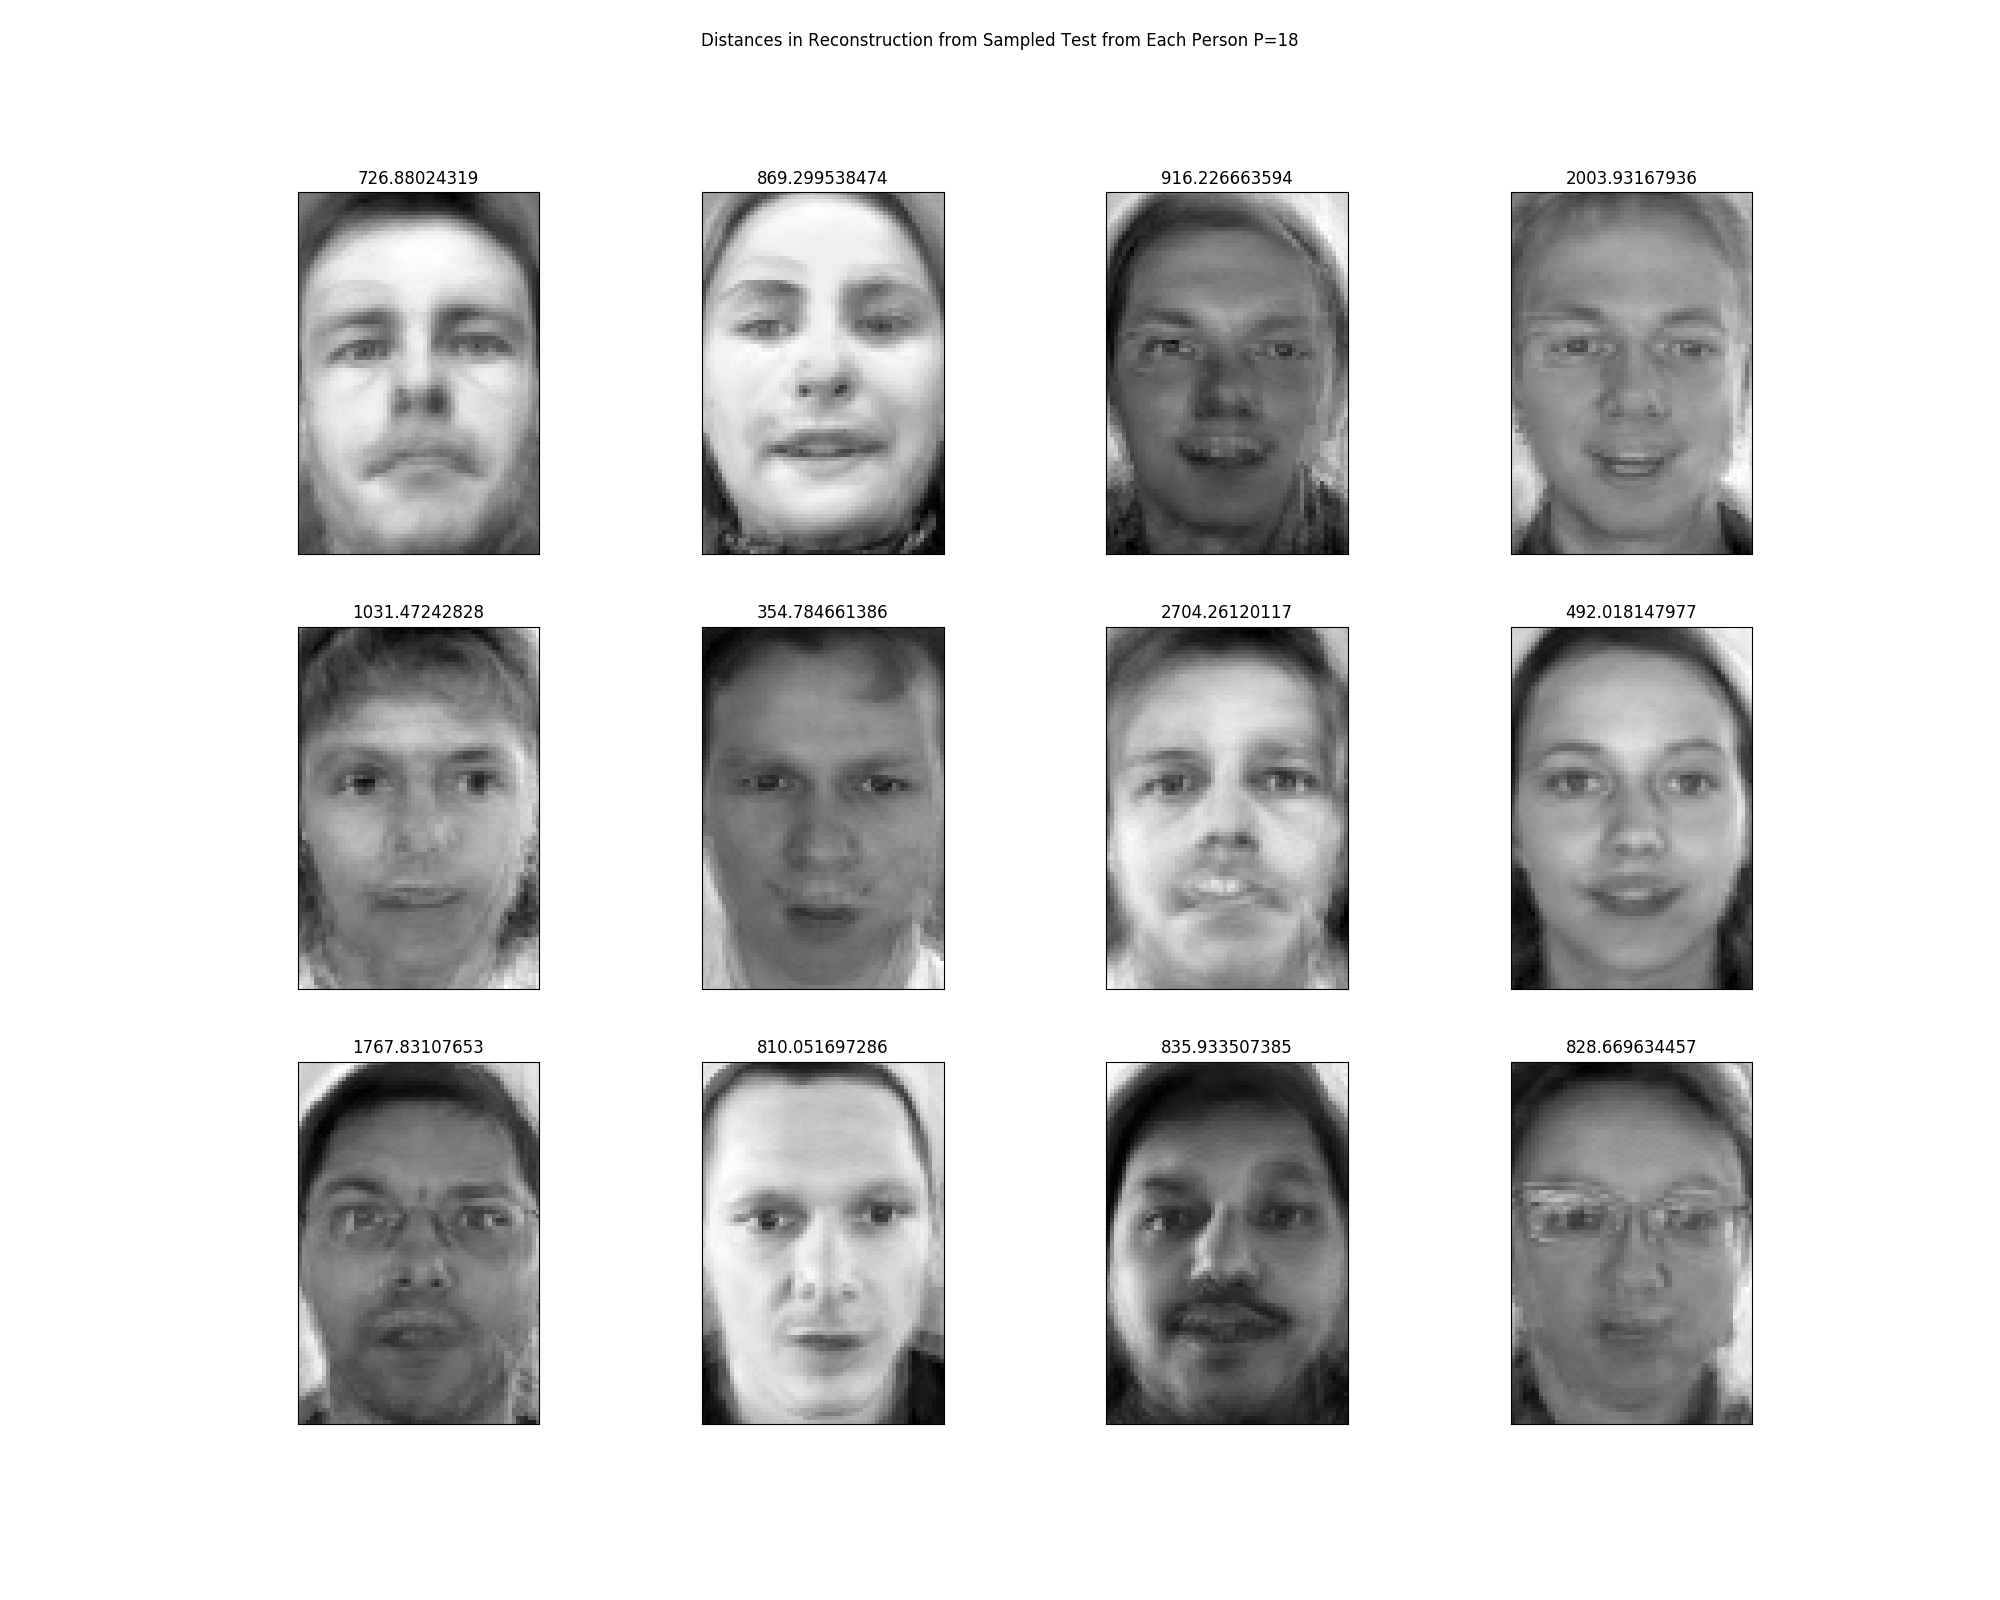
\includegraphics[width=.95\textwidth]{reconstruction_cost_18.png}
\end{figure}
\end{frame}


\begin{frame}
\frametitle{Reconstruction Cost Unknown Face P=9}
\begin{figure}
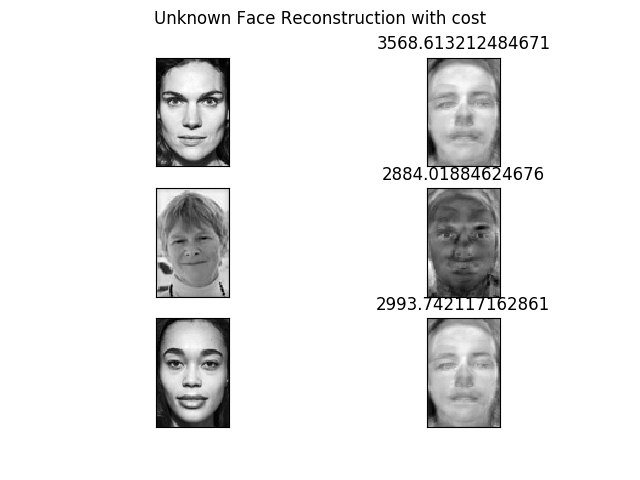
\includegraphics[width=.95\textwidth]{Unknown_Face_cost_P_9.png}
\end{figure}
\end{frame}

\begin{frame}
\frametitle{Reconstruction Cost Unknown Face P=18}
\begin{figure}
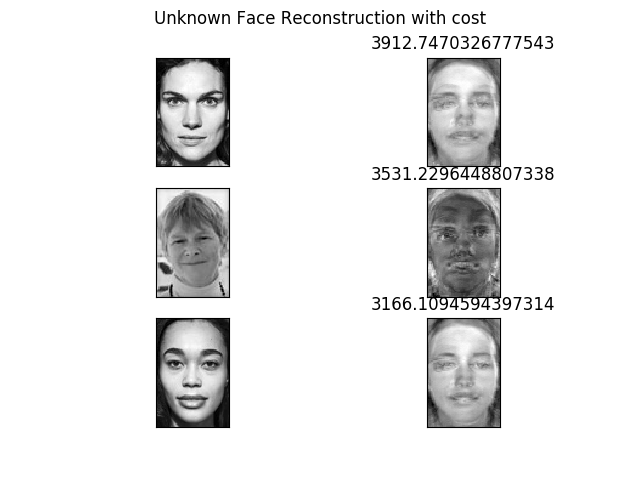
\includegraphics[width=.95\textwidth]{Unknown_Face_cost_P_18.png}
\end{figure}
\end{frame}

\begin{frame}
\frametitle{Reconstruction Cost Non Face P=9}
\begin{figure}
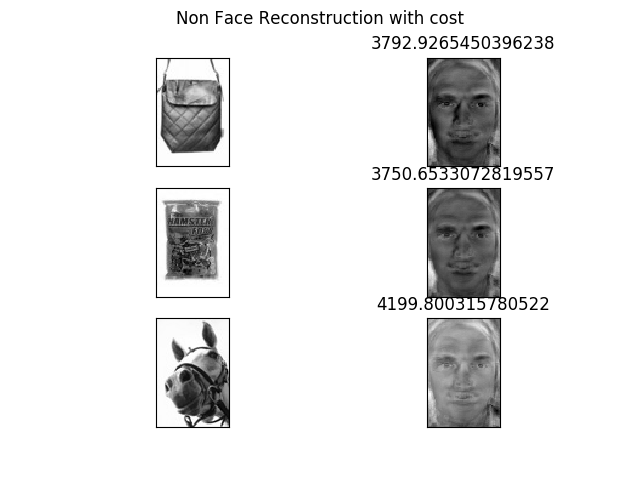
\includegraphics[width=.95\textwidth]{Non_Face_cost_P_9.png}
\end{figure}
\end{frame}

\begin{frame}
\frametitle{Reconstruction Cost Non Face P=18}
\begin{figure}
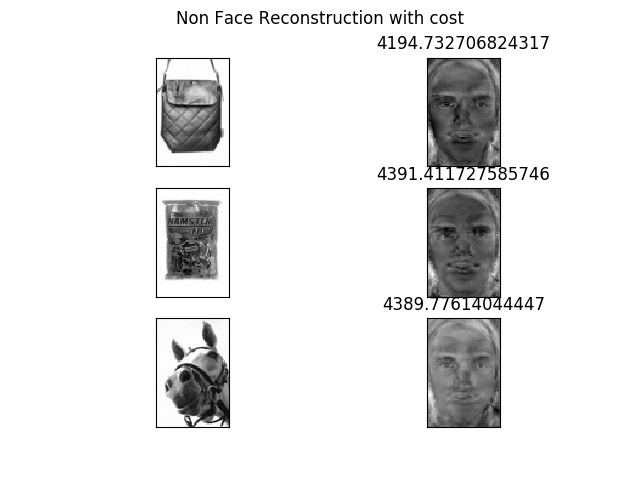
\includegraphics[width=.95\textwidth]{Non_Face_cost_P_18.png}
\end{figure}
\end{frame}

\begin{frame}
\frametitle{Analysis the cost for threshold P=9}
\begin{figure}
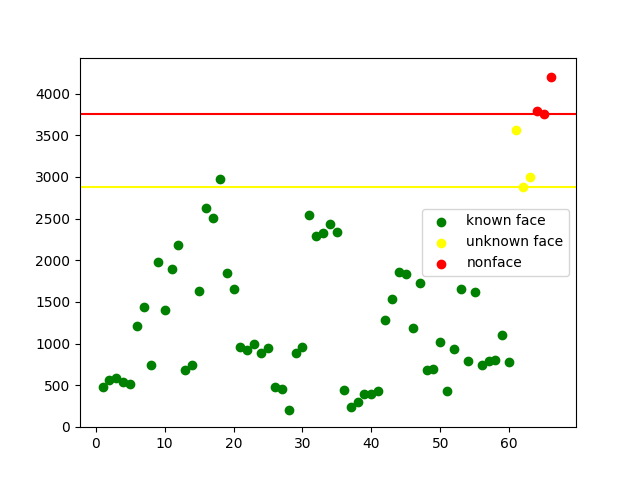
\includegraphics[width=.7\textwidth]{thresholds_9.png}
\caption{The cost for known face, unknown face and Non face are distinct. 
So we have used threshold for classifying images to these category based on the thresh hold. 
This scatter plot Shows all the test images cost in green dots. The horizontal lines denotes the thresholds}
\end{figure}
\end{frame}

\begin{frame}
\frametitle{Analysis the cost for threshold P=18}
\begin{figure}
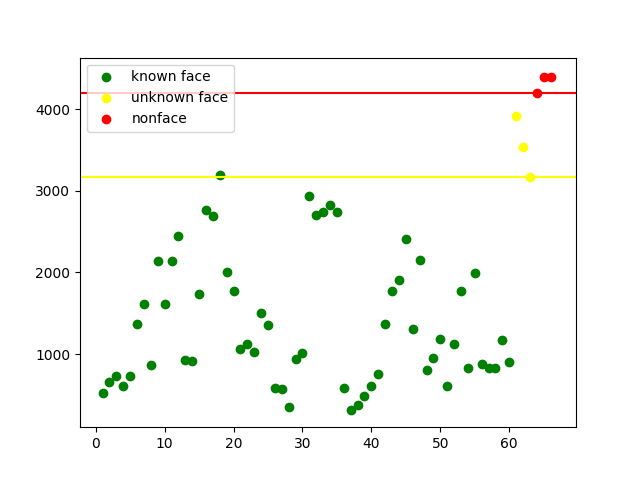
\includegraphics[width=.7\textwidth]{thresholds.png}
\caption{The cost for known face, unknown face and Non face are distinct. 
So we have used threshold for classifying images to these category based on the thresh hold. 
This scatter plot Shows all the test images cost in green dots. The horizontal lines denotes the thresholds}
\end{figure}
\end{frame}


\section{Rank Matrix}

\begin{frame}
\frametitle{Classification Rank Matrix on Test Data}
\begin{table}
  \resizebox{.35\linewidth}{!}{%change the size of the table
  \noindent\pgfplotstabletypeset[% Use noindent
     % column type=,   % dec sep align, % fixed zerofill, 
     % WARNING!!! Above commands may cause miss alignment in multicolumn
     precision=0,
     col sep=space,
     every head row/.style={
        before row={%
          \toprule%
          \multicolumn{1}{|c|}{$\bigstar$} & \multicolumn{2}{|c|}{Ranks (\%)}\\%
          \toprule
        },
        after row={
          \midrule
        }
     },
     columns/0/.style ={column name=Person, column type=|c|},
     columns/1/.style ={column name=1},
     columns/2/.style ={column name=2, column type=c|},
     every last row/.style={after row=\bottomrule},
     ]{rank_mat_P_3.csv}
  }
  \caption{Rank Matrix P=3}
\end{table}
\end{frame}

\begin{frame}
\frametitle{Classification Rank Matrix on Test Data}
\begin{table}
  \resizebox{.4\linewidth}{!}{%change the size of the table
  \noindent\pgfplotstabletypeset[% Use noindent
     % column type=,   % dec sep align, % fixed zerofill, 
     % WARNING!!! Above commands may cause miss alignment in multicolumn
     precision=0,
     col sep=space,
     every head row/.style={
        before row={%
          \toprule%
          \multicolumn{1}{|c|}{$\bigstar$} & \multicolumn{3}{|c|}{Ranks (\%)}\\%
          \toprule
        },
        after row={
          \midrule
        }
     },
     columns/0/.style ={column name=Person, column type=|c|},
     columns/1/.style ={column name=1},
     columns/2/.style ={column name=2},
     columns/3/.style ={column name=3, column type=c|},
     every last row/.style={after row=\bottomrule},
     ]{rank_mat_P_9.csv}
  }
  \caption{Rank Matrix P=9}
\end{table}
\end{frame}

\begin{frame}
\frametitle{Classification Rank Matrix on Test Data}
\begin{table}
  \resizebox{.4\linewidth}{!}{%change the size of the table
  \noindent\pgfplotstabletypeset[% Use noindent
     % column type=,   % dec sep align, % fixed zerofill, 
     % WARNING!!! Above commands may cause miss alignment in multicolumn
     precision=0,
     col sep=space,
     every head row/.style={
        before row={%
          \toprule%
          \multicolumn{1}{|c|}{$\bigstar$} & \multicolumn{3}{|c|}{Ranks (\%)}\\%
          \toprule
        },
        after row={
          \midrule
        }
     },
     columns/0/.style ={column name=Person, column type=|c|},
     columns/1/.style ={column name=1},
     columns/2/.style ={column name=2},
     columns/3/.style ={column name=3, column type=c|},
     every last row/.style={after row=\bottomrule},
     ]{rank_mat_P_18.csv}
  }
  \caption{Rank Matrix P=18}
\end{table}
\end{frame}

\begin{frame}
\frametitle{Classification Rank Matrix on Test Data}
\begin{table}
  \resizebox{.4\linewidth}{!}{%change the size of the table
  \noindent\pgfplotstabletypeset[% Use noindent
     % column type=,   % dec sep align, % fixed zerofill, 
     % WARNING!!! Above commands may cause miss alignment in multicolumn
     precision=0,
     col sep=space,
     every head row/.style={
        before row={%
          \toprule%
          \multicolumn{1}{|c|}{$\bigstar$} & \multicolumn{3}{|c|}{Ranks (\%)}\\%
          \toprule
        },
        after row={
          \midrule
        }
     },
     columns/0/.style ={column name=Person, column type=|c|},
     columns/1/.style ={column name=1},
     columns/2/.style ={column name=2},
     columns/3/.style ={column name=3, column type=c|},
     every last row/.style={after row=\bottomrule},
     ]{rank_mat_P_72.csv}
  }
  \caption{Rank Matrix P=72}
\end{table}
\end{frame}

\begin{frame}
\frametitle{Conclusion}
\begin{itemize}
  \item The overall accuracy on test set was 91.66\%
  \item The threshold values has been found to be distinctive for known, unknown face and non face
  \item Upside down rotation of an known face could not be recognized using this model.
  \item In fact PCA is often sensitive to translation of the face
  \item For example Person 2 was hard to recognize because of the translation of the face
  \item The reason is the underlining assumption of PCA of components are linear
  \item However in feature space translation may not result in linear transformation
  \item One obvious fix to this specific test case can be fixing the image by aligning with rest of the the training images
  \item For a better solution one may try more advanced features and/or algorithm like Neural Network.
\end{itemize}
\end{frame}


% ------------------------------------------------------------------------------------------------------------------

\end{document}

